\begin{enumerate}
	\item An office has 4 copying machine, and the random variable X measures how many of them are in use at a particular moment in time. Suppose that $P(X = 0) = 0.08$, $P(X = 1) = 0.11$, $P(X = 2) = 0.27$ and $P(X = 3) = 0.33$.
	\begin{enumerate}
		\item What is $P(X = 4)$?
		\begin{multline*}
			P(X = 4) = 1-P(X=3)-P(X=2)-P(X=1)-P(X=0)\\
			=1-0.33-0.27-0.11-0.08=0.21
		\end{multline*}
		\item Draw a line graph of the probability mass function.
		\begin{center}
			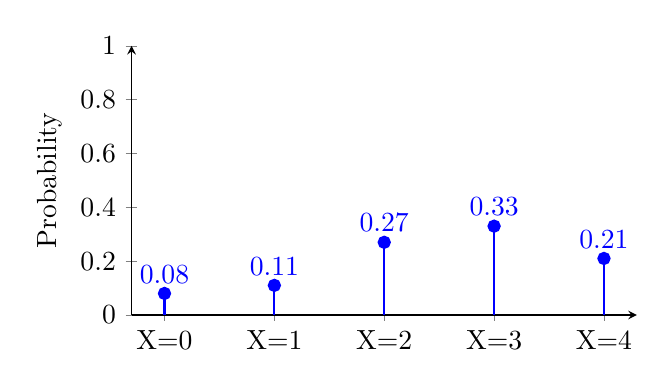
\begin{tikzpicture}
			\pgfkeys{/pgf/number format/fixed}
			\begin{axis}[
				ybar,
				xmin=-0.3, xmax=4.3,
				axis lines=left,
				ylabel={Probability},
				xtick={0,1,2,3,4},
    			xticklabels={{X=0},{X=1},{X=2},{X=3},{X=4}},
				ymin = 0, ymax = 1,
				ytick = {0,0.2,...,1},
				nodes near coords,
				nodes near coords align={vertical},
				width=8cm,height=5cm
				]
			\addplot[ycomb, thick, blue, mark=*] coordinates {(0,0.08) (1,0.11) (2,0.27) (3,0.33) (4,0.21)};
			\end{axis}
			\end{tikzpicture}
		\end{center}
		\item Construct and plot the cumulative distribution function.\\
		The cumulative distribution function:
		$\displaystyle F(x) = \left\{\begin{array}{ll}
		0.08 & 0\le x<1 \\
			0.19 & 1\le x<2 \\
			0.46 & 2\le x<3 \\
			0.79 & 3\le x<4 \\
			1 & x = 4 \\
		\end{array}\right.$
		Plot of the cumulative distribution function:
		\begin{center}
			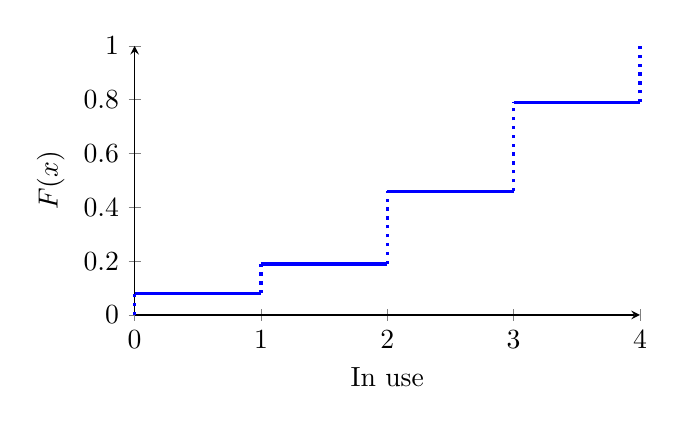
\begin{tikzpicture}
			\pgfkeys{/pgf/number format/fixed}
			\begin{axis}[
				axis lines=left,
				xlabel={In use},
				ylabel={$F(x)$},
				xtick={0,1,2,3,4},
				ytick={0,0.2,...,1},
				clip = false,
				width=8cm,height=5cm
			]
			\addplot[
				empty line=jump,
				const plot,very thick, blue
			] coordinates {
				(0,0.08)
				(1,0.08)

				(1,0.19)
				(2,0.19)

				(2,0.46)
				(3,0.46)
				
				(3,0.79)
				(4,0.79)
			};
			\addplot[
				const plot,very thick, dotted,
				empty line=jump, blue
			] coordinates {
				(0,0)
				(0,0.08)

				(1,0.08)
				(1,0.19)

				(2,0.19)
				(2,0.46)

				(3,0.46)
				(3,0.79)

				(4,0.79)
				(4,1)
			};
			\end{axis}
			\end{tikzpicture}
		\end{center}
		\item  What is the expected number of copying machines at a particular moment in time?
		\begin{multline*}
			E(X)=0+P(X=1)+2P(X=2)+3P(X=3)+4P(X=4)\\
			= 0.11 + 2\times0.27 + 3\times0.33 + 4\times 0.21 = 2.48 (\n{copying machine})
		\end{multline*}
		\item Calculate the variance and standard deviation of the number of copying machines in use at a particular moment.
		\begin{multline*}
			\n{Var}(X) = \sum_{i = 0}^{4}{x(x-E(x))^2}\\ =0.08(0-2.48)^2 + 0.11(1-2.48)^2+ 0.27(2-2.48)^2 + 0.33(3-2.48)^2 + 0.21(4-2.48)^2 = 1.3696
		\end{multline*}
		$$\sigma = \sqrt{1.3696} \approx 1.1702991071 $$
	\end{enumerate}
	\item  fair coin is tossed 3 times. A player wins \$1 if the first toss is a head, but loses \$1 if the first toss is a tail. Similarly, the player wins \$2 if the second toss is a head, but loses \$2 if the second toss is a tail, and wins or loses \$3 according to the result of the third toss.\\
	Let the random variable X be the total winnings after the 3 tosses (possibly a negative value if losses are incurred).
	\begin{enumerate}
		\item Construct the probability mass function.\\
		Let $(x,y,z)$ be the result of the throws where $x,y,z$ are $1$ for win, and $0$ for lost of the 1st, 2nd, 3rd throw respectively.\\
		Let $W(x,y,z)$ be the winnings (\$) of result $(x,y,z)$.\\
		Calculate $W$:
		\begin{align*}
			W(0,0,0)=-6&&W(1,0,0)=-4&&W(0,1,0)=-2&&W(1,1,0)=0\\
			W(1,1,1)=6&&W(0,1,1)=4&&W(1,0,1)=2&&W(0,0,1)=0
		\end{align*}
		Since the events are equally likely,
		$$P(x) = \left\{\begin{array}{ll}
			1/8 & x=-6\\
			1/8 & x=-4\\
			1/8 & x=-2\\
			1/4 & x=0 \\
			1/8 & x=2\\
			1/8 & x=4\\
			1/8 & x=6\\
		\end{array}\right.$$
		\item Construct the cumulative distribution function.
		$$F(x) = \left\{\begin{array}{ll}
			1/8 & -6\le x < -4\\
			1/4 & -4\le x < -2\\
			3/8 & -2\le x < 0\\
			5/8 & 0\le x < 2\\
			3/4 & 2\le x < 4\\
			7/8 & 4\le x < 6\\
			1 & x=6\\
		\end{array}\right.$$
		\item What is the most likely value of the random variable X?
		The most likely value of $X$ is $0$.
	\end{enumerate}
	\item The figure presents the cumulative distribution function of a random variable. Make a table and line graph of its probability mass function.\\
	Probability mass function:
	\begin{center}
		\begin{tabular}{|c|c|}
			\hline
			& P(X)\\
			\hline
			-4 & 0.21\\ 
			-1 & 0.11\\
			0 & 0.07\\
			2 & 0.29\\
			3 & 0.13\\
			7 & 0.19\\
			otherwise & 0\\
			\hline
		\end{tabular}
	\end{center}
	Line graph of the probability mass function:
	\begin{center}
		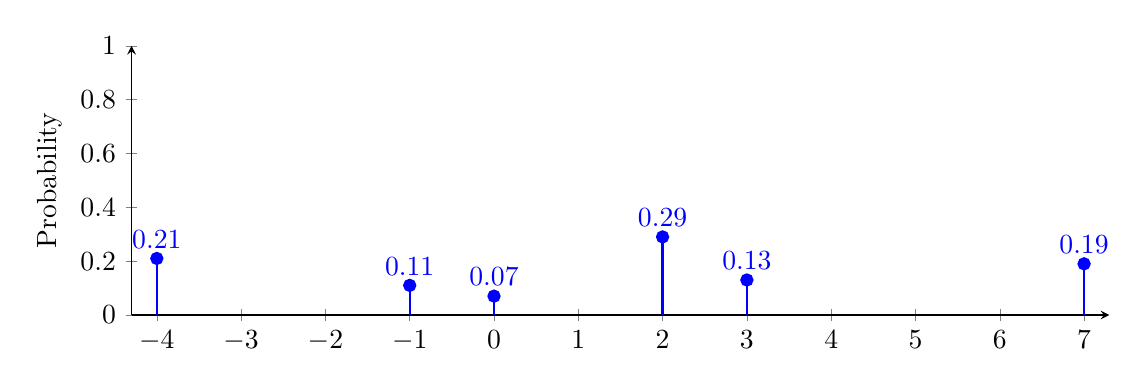
\begin{tikzpicture}
		\pgfkeys{/pgf/number format/fixed}
		\begin{axis}[
			ybar,
			axis lines=left,
			xmin=-4.3, xmax=7.3,
			xtick={-4,-3,...,7},
			ylabel={Probability},
			ymin = 0, ymax = 1,
			ytick = {0,0.2,...,1},
			nodes near coords,
			nodes near coords align={vertical},
			width=14cm,height=5cm
			]
		\addplot[ycomb, thick, blue, mark=*] coordinates {(-4,0.21) (-1,0.11) (0,0.07) (2,0.29) (3,0.13) (7,0.19)};
		\end{axis}
		\end{tikzpicture}
	\end{center}
\end{enumerate}
